\chapter{Testing and Result}\label{ch:testing}

\section{Introduction}\label{sec:testingIntroduction}

This chapter provides an overview of the testing scenarios associated with the \textbf{Collective} mobile journaling application. The importance of testing in the software development life cycle is paramount, as it ensures that the system operates reliably and meets user requirements. The primary goal of testing is to identify and resolve technical issues and bugs, ensuring the system functions correctly and aligns with the specified requirements outlined in Chapter~\ref{ch:methodology}.

Testing the Collective mobile journaling application involves evaluating the system's various functionalities including journal entry creation, user authentication, data storage and synchronization, AI-powered insights, and offline capabilities. Due to the complexity of the mobile application and the numerous possible input and output combinations across different Android devices, it is impractical to test every possible scenario. However, thorough testing aims to cover as many scenarios as possible to ensure robustness and reliability.

The chapter emphasizes four critical testing methodologies: \textbf{Integration Testing} to verify component interaction, \textbf{System Testing} to validate overall functionality, \textbf{User Acceptance Testing} with test cases specified in individual tables, and \textbf{Usability Testing} conducted through structured feedback gathering with respondents as testers. By adhering to these testing standards, the chapter aims to demonstrate how the Collective mobile journaling application meets quality standards and fulfills user requirements.

\section{Test Objective}\label{sec:testObjective}

The test plan focuses on identifying and documenting as many bugs as possible to enhance the system's reliability. The \textbf{Collective} mobile journaling application underwent extensive testing through four testing phases: Integration Testing to verify component interactions, System Testing to validate complete functionality, User Acceptance Testing with test cases documented in individual tables, and Usability Testing conducted through structured feedback gathering with respondents as testers.

The application testing focused on crucial operations such as journal entry creation, editing, deletion, user authentication, data synchronization, and AI-powered insights generation. The user interface has been carefully crafted to ensure ease of use, facilitating smooth navigation throughout the journaling experience. Throughout the development process, emphasis has been placed on performance and usability to ensure a seamless journaling experience.

\section{Test Process}\label{sec:testProcess}

Figure~\ref{fig:test-process} illustrates the Test Process approach as follows:

\textbf{i. 60\% development progress:} At this stage, the majority of core features are implemented including Flutter framework setup, Firebase authentication, journal entry creation, AI-powered insights integration, and basic offline functionality. This milestone provides sufficient functionality for initial integration testing.

\textbf{ii. Integration Testing:} With core components developed, integration testing begins to verify that different modules work together seamlessly. This includes testing the integration between Firebase authentication, local database storage with Sembast, AI service connectivity with DeepSeek API, and user interface elements to ensure effective communication between components.

\textbf{iii. 80\% development progress:} Following successful integration testing, development continues with advanced features such as enhanced offline synchronization, media attachment capabilities, analytics dashboard, and bookmark management functionality.

\textbf{iv. System Testing:} At this development milestone, comprehensive system testing evaluates the entire Collective mobile journaling application to verify that all specifications and requirements are met. Both functional and non-functional aspects, such as performance, offline functionality, and data synchronization, are thoroughly tested across different Android devices.

\textbf{v. 95\% development progress:} With system testing completed and major issues resolved, the application reaches near-completion status with all critical features implemented and tested, ready for final user validation.

\textbf{vi. User Acceptance Testing:} At this advanced stage, the system undergoes comprehensive test case validation covering all functional requirements. Individual test cases are documented in dedicated tables to ensure systematic coverage of all system features and user scenarios.

\textbf{vii. Usability Testing:} In this final phase, the nearly complete system undergoes usability evaluation through structured feedback gathering with respondents as testers. The Collective mobile journaling application must demonstrate ease of use and user satisfaction to validate its core objective of providing a simplified, distraction-free digital journaling experience.

\begin{figure}[H]
\centering
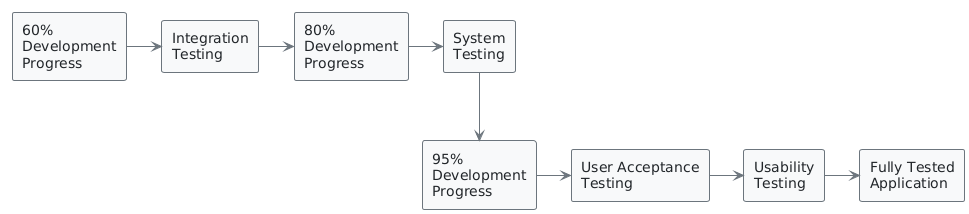
\includegraphics[width=0.8\textwidth]{files/imgs/test_process_flow.png}
\caption{Test Process Flow for Collective Mobile Journaling Application}
\label{fig:test-process}
\end{figure}

\subsection{Risk and Contingencies}\label{sec:riskContingencies}

Several risk-related issues need to be addressed with contingency during testing as they could lead to major troublesome problems that will affect testing development. There are project and product risks; for product risks, they will be specified in risk-based testing sections, while here are the project risks for the Collective mobile journaling application testing:

\begin{table}[H]
\centering
\caption{Risks and Contingencies for Collective Mobile Journaling Application Testing}
\label{tab:risks-contingencies}
\begin{tabular}{|p{1cm}|p{4cm}|p{3cm}|p{6cm}|}
\hline
\textbf{ID NO} & \textbf{Project Risks} & \textbf{Impact} & \textbf{Contingencies} \\
\hline
1 & Unavailability of Android test devices & Unable to run mobile tests and delay testing schedule & Proper planning and preparing checklist to ensure all Android devices are available. If event occurs, use emulators or request additional devices from colleagues. \\
\hline
2 & Firebase backend service downtime & Unable to test authentication, cloud sync, and data storage features & Implement local testing environment with mock Firebase services. Schedule tests during stable service hours and have backup testing scenarios. \\
\hline
3 & DeepSeek API rate limiting or service unavailability & Cannot test AI-powered insights and analysis features & Implement mock AI responses for testing. Cache previous API responses for test scenarios. Consider alternative AI service testing. \\
\hline
4 & Internet connectivity issues & Unable to test online features, cloud synchronization, and API integrations & Focus on offline functionality testing first. Use mobile hotspot as backup connection. Prepare test scenarios for both online and offline modes. \\
\hline
5 & Time and resource limitations & Not enough time to complete comprehensive testing across all features & Prioritize critical path testing and core functionalities. Eliminate low-priority test cases. Focus on integration and system testing for essential features. \\
\hline
6 & Large number of defects found during integration testing & Unable to proceed with system and user acceptance testing & Implement defect triage system. Fix critical defects first. Parallel testing and development approach for non-blocking issues. \\
\hline
7 & Lack of real user data for testing & Test scenarios may not reflect actual usage patterns & Generate realistic test data based on user research. Recruit beta testers for realistic data creation. Use anonymized sample journal entries. \\
\hline
8 & Changes in Flutter framework or Firebase SDK versions & Compatibility issues affecting test environment stability & Maintain version control and testing on multiple framework versions. Keep rollback options available. Document version-specific test procedures. \\
\hline
9 & Insufficient knowledge of mobile testing tools and methodologies & Delayed testing process and potential test inaccuracy & Consult with mobile development experts and supervisor. Conduct training on Flutter testing frameworks. Research mobile testing best practices. \\
\hline
10 & User recruitment challenges for usability testing & Limited or biased feedback for user acceptance and usability evaluation & Expand recruitment channels including social media and university networks. Offer incentives for participation. Use remote testing tools if needed. \\
\hline
\end{tabular}
\end{table}